Since
\begin{align}
%    \vec{x}^T \myvec{\sqrt{5} & 0\\0 & 0}\vec{x} + 2\myvec{\frac{1}{2} & 0}\vec{x} + \sqrt{5} = 0\\
    \sqrt{5}x^2 + x + \sqrt{5} = 0\\
%     x^2 + \frac{1}{\sqrt{5}}x + 1 = 0\\
%     x^2 + \frac{1}{\sqrt{5}}x + \brak{\frac{1}{2\sqrt{5}}}^2 - \brak{\frac{1}{2\sqrt{5}}}^2 + 1 = 0\\
%     \brak{x + \frac{1}{2\sqrt{5}}}^2 + 1 - \frac{1}{20} = 0\\
\implies    \brak{x + \frac{1}{2\sqrt{5}}}^2 + \frac{19}{20} = 0,
\end{align}
the equation has no real roots.
%
% The given expression  can be represented in the vector form as
% \begin{align}
%     y = \vec{x}^T \myvec{\sqrt{5} & 0\\0 & 0}\vec{x} + 2\myvec{\frac{1}{2} & 0}\vec{x} + \sqrt{5}
% \end{align}
% where 
% \begin{align}
%     \vec{x} = \myvec{x\\0}
% \end{align}
% Subsituting $y = 0$, we get:
% \begin{align}
%     \vec{x}^T \myvec{\sqrt{5} & 0\\0 & 0}\vec{x} + 2\myvec{\frac{1}{2} & 0}\vec{x} + \sqrt{5} = 0\\
%     \sqrt{5}x^2 + x + \sqrt{5} = 0\\
%     x^2 + \frac{1}{\sqrt{5}}x + 1 = 0\\
%     x^2 + \frac{1}{\sqrt{5}}x + \brak{\frac{1}{2\sqrt{5}}}^2 - \brak{\frac{1}{2\sqrt{5}}}^2 + 1 = 0\\
%     \brak{x + \frac{1}{2\sqrt{5}}}^2 + 1 - \frac{1}{20} = 0\\
%     \brak{x + \frac{1}{2\sqrt{5}}}^2 + \frac{19}{20} = 0
% \end{align}
% Clearly, for no value of $x$ would we get the value of this expression to be $0$, and hence, this equation has no real roots.\\
% The roots can be verified using the python code. As we can see from the graph, $\sqrt{5}x^2 + x + \sqrt{5} = 0$ does not intersect the x-axis anywhere, and hence, has no real roots.\\

%\textbf{Affine Transformation}

Consider $y = \sqrt{5}x^2 + x + \sqrt{5}$, which can be written in the vector form as
%
\begin{align}
\vec{x}^T \myvec{\sqrt{5} & 0\\0 & 0}\vec{x} + 2\myvec{\frac{1}{2} & \frac{-1}{2}}\vec{x} + \sqrt{5} = 0\\
\vec{V} = \myvec{\sqrt{5} & 0\\0 & 0} , \vec{u} = \myvec{\frac{1}{2}\\ \frac{-1}{2}} , f = \sqrt{5}
\end{align}
%
For obtaining the affine transformation, we use:
\begin{align}
    \vec{x} = \vec{P}\vec{y} + \vec{c}
\end{align}
The corresponding eigenvalues of $\vec{V}$ are:
\begin{align}
    \lambda_1 = 0 , \lambda_2 = \sqrt{5}\\
    \vec{D} = \myvec{0 & 0\\0 & \sqrt{5}}
\end{align}
The corresponding eigenvectors are:
\begin{align}
    \vec{p}_1 = \myvec{0\\1} , \vec{p}_2 = \myvec{1\\0}\\
    \vec{P} = \myvec{\vec{p}_1 & \vec{p}_2} = \myvec{0 & 1\\1 & 0}
\end{align}
%
Since $\abs{\vec{V}} = 0$, the given curve is a parabola and is plotted in Fig. \ref{sep/2/23/fig} using
\begin{align}
    \myvec{\vec{u}^\top+\eta \vec{p}_1^\top\\\vec{V}}\vec{c} &= \myvec{-f\\\eta \vec{p}_1-\vec{u}}\\
    \eta &= \vec{u}^\top \vec{p}_1\\
    \implies \eta &= \frac{-1}{2}\\
    \implies \myvec{\frac{1}{2}&-1\\\sqrt{5}&0\\0&0}\vec{c} &= \myvec{-\sqrt{5}\\\frac{-1}{2}\\0}\\
    \implies \vec{c} &= \myvec{\frac{-1}{2\sqrt{5}}\\\frac{19}{4\sqrt{5}}}
\end{align}
As we can see from the graph, the curve does not intersect the x-axis anywhere, and hence, has no real roots.
 \begin{figure}[!ht]
\centering
 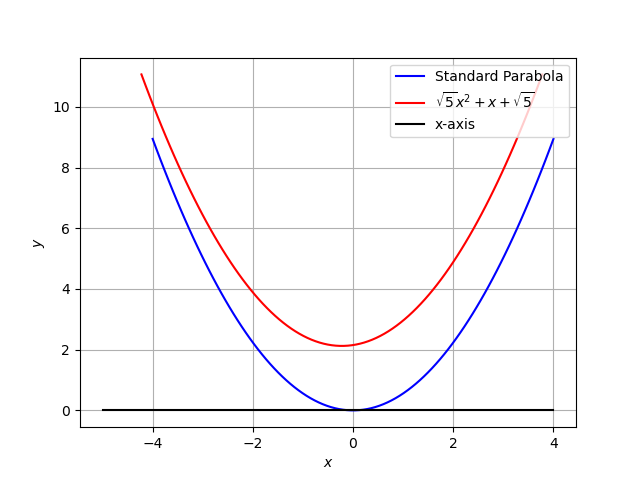
\includegraphics[width=\columnwidth]{solutions/sep/2/23/graph.png}
 \caption{Graph of $ y = \sqrt{5}x^2 + x + \sqrt{5} $}
 \label{sep/2/23/fig}
 \end{figure}

